% -*- TeX-master: "../fat_manual.tex" -*-

\section{System and amplifiers}
The connections from the top of the system are as follows
\begin{center}
  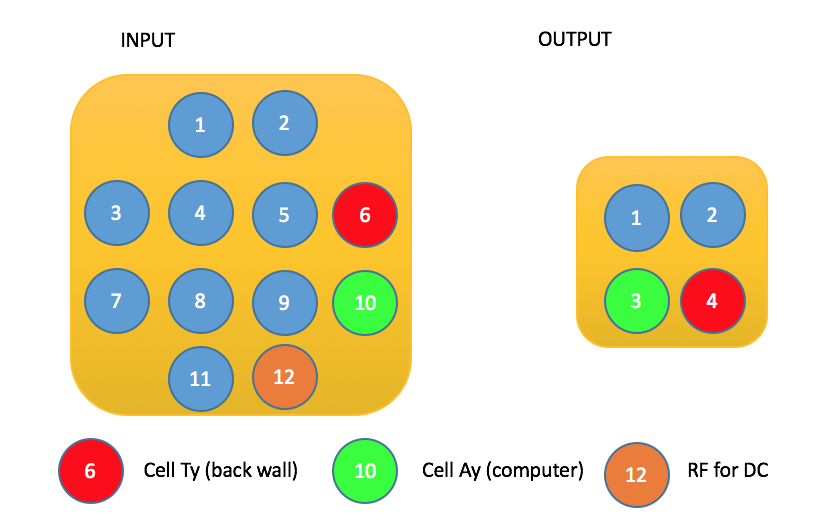
\includegraphics[height=5cm]{top}
  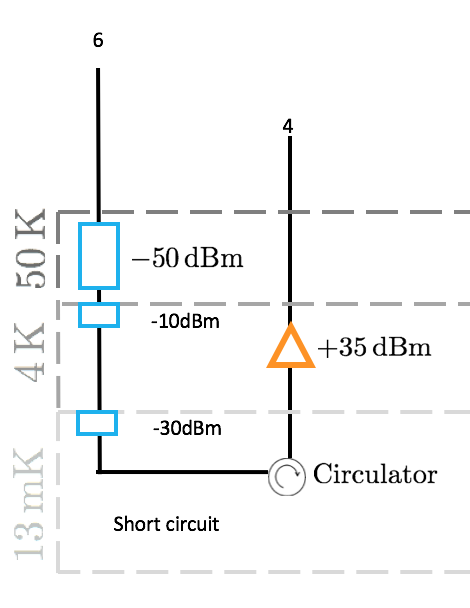
\includegraphics[height=5cm]{side}
\end{center}

\noindent The attenuator markings, which  are attached to the various
plate,   have    the   last   number   depicting    the   atuniation.
\red{\textbf{Note, that it can be 0dB!!!}}
\begin{center}
  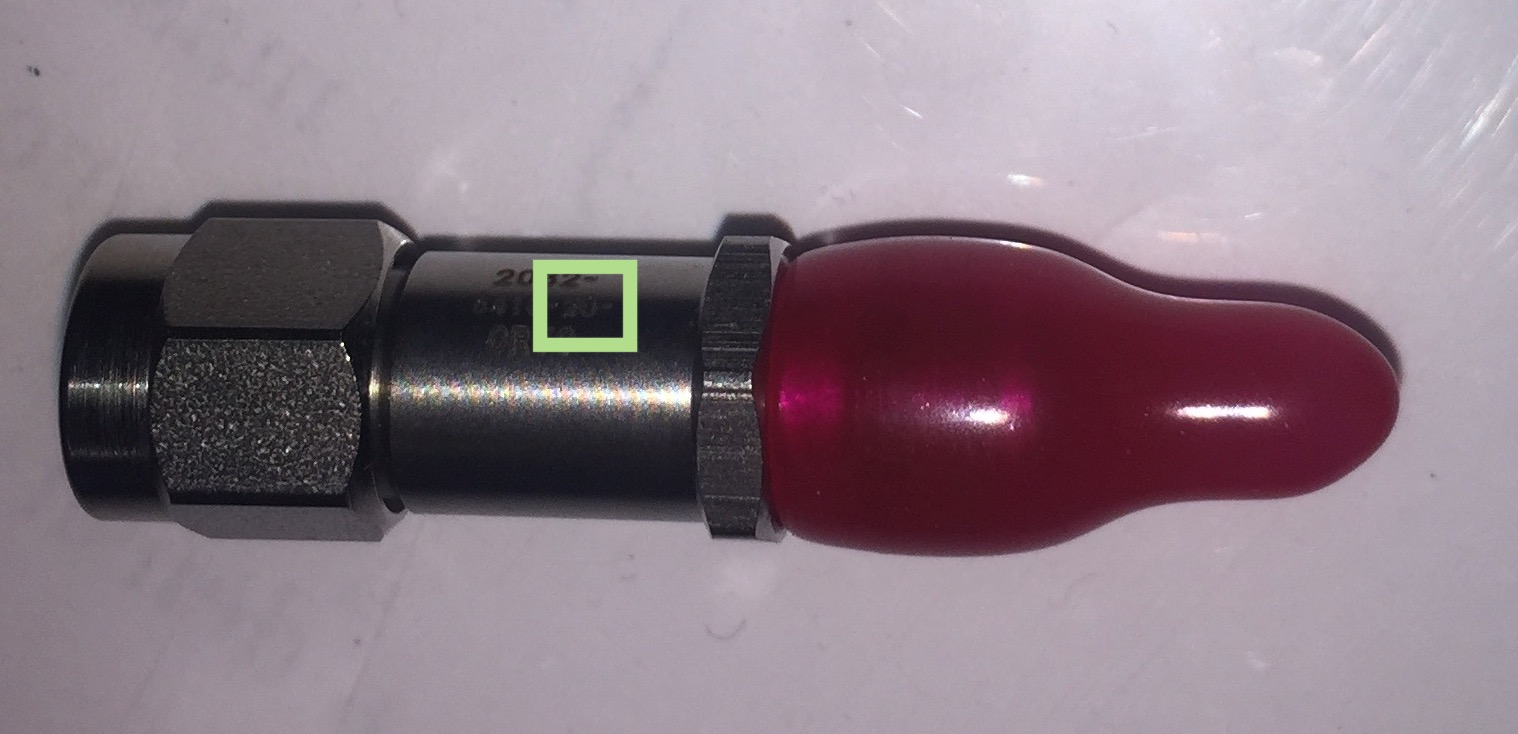
\includegraphics[height=5cm]{filter}
\end{center}

\begin{framed}\noindent
  \red{\textbf{\Large Turn amplifiers off when handling them!}}
\end{framed}

In order to turn  both the room temp and cold  amplifiers on, we need
to apply voltages
\begin{enumerate}
\item
  \href{http://www.lownoisefactory.com/products/roomtemp/1-15-ghz/}{\textbf{LNF-LNR1\_15A}}
  Climb up on the ladder \ira turn  the power supply on \ira turn the
  small  \quote{on}  buttons  at  the bottom  of  the  amplifier  to
  \quote{on} at the same time;
  \[
    \text{Left display:} 2.44V \quad \text{Right display:}2.67\,\text{V}
  \]
\item There are two {LNF-LNR1\_15A} amplifiers:
  \begin{itemize}
  \item Input 10, Output 3, Cell Ay, 337\,V, closer to computer;
  \item Input 6, Output 4, Cell Ty, 330V, closer to back wall;
  \end{itemize}
  On each line there  is a 50dB attenuator in the  top hood, 10dBm on
  the 4K plate  (first grey plate), 30dB on the  13mK plate.  Turn on
  the correct switch on the grey box;
\item                                                              My
  \href{http://www.atlantecrf.com/products/active_components/amplifiers/wide_band_amplifiers.htm}{AOX-010120 amplifier}
  just needs 5\,V from any supply.
\end{enumerate}
\newpage
